\section{Survey}
\subsection{Real-time tasks \& schedulers}
\begin{frame}
  \frametitle{Real-time tasks}
  \begin{definition}
    Real-time tasks are the independant or co-dependant units of
    execution that may handle different aspects or axes of the entire
    computational responsibility imposed upon the system under
    separate temporal constraints
  \end{definition}
  \pause 
  \begin{itemize}
    \item{Real-time tasks are almost always recurrent, in that they
      occur iteratively over the lifetime of the system and one
      \emph{instance} of a task is called a \emph{job}}
    \item{Tasks are, in effect, containers for jobs or functionality}
  \end{itemize}
\end{frame}

\frame {
  \frametitle{Temporal characteristics of tasks}
  \begin{itemize}
    \item{\textbf{Dispatch protocol:} Time triggered or event
      triggered}
    \item{\textbf{Period (T):} The frequency of time triggered tasks}
    \item{\textbf{Deadline (D):} The instance of time between dispatch
      and completion of a job in nominal functioning of the system}
    \item{\textbf{WCET (C):} Worst Case Execution Time for \emph{any}
      job of a task}
  \end{itemize}
  \pause
  \begin{definition}
    Task \alert{dispatch} is when it is taken from the set of blocked
    tasks and added to the set of ready tasks
  \end{definition}

  \begin{definition}
    Task \alert{release} is when the task is taken from the ready
    queue and put on the processor itself, and thus starts execution
  \end{definition}
}

\frame {
  \frametitle{Time-triggered or periodic tasks}
  \begin{itemize}
    \item{Those that are dispatched as a function of system time}
    \item{Temporal characteristic of \alert{period}}
    \item{Are mostly hard real-time tasks}
    \item{Major uses include
      \begin{enumerate}
        \item{In control systems, periodic tasks carry out the
          computation of the \alert{transfer function}}
        \item{In both control and information/monitoring systems, they
          are used to periodically read sensors}
        \item{Status display updates to provide important information
          to operators}
      \end{enumerate}
    }
  \end{itemize}
}

\frame {
  \frametitle{Event-triggered or aperiodic tasks}
  \begin{itemize}
    \item{Aperiodic tasks are those that are dispatched as a result of
      an event from the environment or another task}
    \item{Aperiodic tasks may overload a system in case of an
      \alert{event storm}}
    \item{Safer version is sporadic task
      \begin{itemize}
        \item{Launched as a function of event arrival \emph{and}
          system time}
        \item{Temporal characteristic of minimum inter-arrival time
          between successive task dispatches}
        \item{Results in a system that is resilient to overload}
      \end{itemize}
    }
    \item{Thus, for safety-critical systems, sporadic tasks are a much
      more attractive option}
  \end{itemize}
}

\frame {
  \frametitle{Real-time schedulers}
  \begin{itemize}
    \item{Scheduler is responsible for task dispatch and release}
    \item{Real-time schedulers make decisions based on temporal
      characteristics of the task set}
    \item{Various real-time schedulers exist
      \begin{itemize}
        \item{Cyclic schedulers}
        \item{Fixed priority preemptive scheduler}
        \item{Earliest deadline first scheduler}
        \item{$\ldots$}
      \end{itemize}
    }
  \end{itemize}
}

\frame {
  \frametitle{Cyclic executives}
  \begin{itemize}
    \item{Oldest real-time scheduling method available}
    \item{Single timer callback calls different functions of the
      system}
    \item{Implies a synchronous system
      \begin{itemize}
        \item{Zero execution time semantics}
        \item{All tasks must be periodic}
        \item{All periods must be harmonic with the \alert{base rate}}
        \item{Assumption that the program reacts to external event
          before other event occurs}
        \item{No preemption, no concurrency control, no race
          conditions}
        \item{Completely deterministic execution}
      \end{itemize}
    }
  \end{itemize}
}

\frame[containsverbatim] {
  \frametitle{Cyclic executives (contd.)}
    \begin{minipage}{0.45\linewidth}
\begin{lstlisting}[language=c]
{
  static int job = 0;
  job++;
  A();
  if(job==2 || job==4) {
    B();
    C();
  }
  if(job==4) {
    D();
    job = 0;
  }
}
\end{lstlisting}
    \end{minipage}
    \hspace{2mm}
    \begin{minipage}{0.45\linewidth}
      $\includegraphics[scale=0.6]{../figs/cyclic_exec}$
    \end{minipage}
}

\frame {
  \frametitle{Process based executives}
  \begin{itemize}
    \item{The ``operating system'' approach}
    \item{Separate processes, each with potentially multiple threads}
    \item{Can be preemptive or non-preemptive}
    \item{Context switching to change tasks on the processor}
    \item{True multi-processing capability}
    \item{Implies a number of things
      \begin{itemize}
        \item{Allows periodic \emph{and} aperiodic tasks}
        \item{Is not restricted to zero execution time semantics}
        \item{Concurrency is possible, thus mutual exclusion required}
        \item{Non-determinism is possible in execution}
      \end{itemize}
    }
    \item{The scheduler decides which task will execute}
  \end{itemize}
}

\frame {
  \frametitle{Fixed Priority Preemptive Scheduling}
  \begin{itemize}
    \item{A simple, robust real-time scheduler}
    \item{The scheduler is launched periodically, and it selects the
      highest priority task among all those that are ready to execute}
    \item{At any time, a lower priority task may be interrupted by a
      higher priority task}
    \item{Task priorities do not change during the lifetime of the
      system}
  \end{itemize}
}

\frame {
  \frametitle{Priority assignments with RMA, RTA}
  \begin{itemize}
    \item{Seminal paper of Leyland \& Liu gives optimum priority
      assignment}
    \item{Rate Monotonic Assignment implies priority assignment in
      inverse order of periods, i.e., fastest task is assigned highest
      priority}
    \item{Basic RMA is for independant tasks, those that do not
      communicate}
    \item{Task interaction can be analyzed by introducing terms in the
      equations (dependant on type of synchronization protocol)}
    \item{More precise (and optimistic) analysis technique or Response
      Time Analysis exists as well}
  \end{itemize}
}

\subsection{Model-driven approaches}

\frame {
  \frametitle{UML}
  \begin{itemize}
    \item{Software design language standardized by the OMG}
    \item{An amalgamation of various methods, OMT, OOSE, Booch}
    \item{It is a large, complex language (13 different diagrams)}
    \item{More or less an elevation of OOP concepts to design level}
    \item{Allows modeling of \alert{classes} and \alert{objects}}
    \item{Important diagrams from the point-of-view of RT systems are
      the class diagram, the statechart and the composite structure
      diagram
      \begin{itemize}
        \item{Class diagrams allow the graphical description of the
          class hierarchy and relation topology among classes}
        \item{Statecharts allow the description of functional behavior
          of classes}
        \item{Composite structure diagrams allow the description of
          hierarchies of composition}
      \end{itemize}
    }
  \end{itemize}
}

\frame {
  \frametitle{UML (contd.)}
  $\includegraphics[scale=0.6]{../figs/class_diag}$
}

\frame {
  \frametitle{UML (contd.)}
  %\begin{minipage}{0.45\linewidth}
    \textbf{Advantages}
    \begin{itemize}
      \item{Standardized, prevalent}
      \item{Close to the software domain}
      \item{Intuitive modeling of OO}
      \item{Intuitive code generation, specially for OO target
        languages}
      \item{Contains extension mechanisms}
    \end{itemize}
  %\end{minipage}
  %\hspace{2mm}
  \pause
  %\begin{minipage}{0.45\linewidth}
    \textbf{Disadvantages}
    \begin{itemize}
      \item{Semantic variation among implementations}
      \item{Very complex}
      \item{Strongly tied to OO concepts!}
      \item{Engages in \alert{semantic overload}}
      \item{No support for hard real-time concepts}
    \end{itemize}
  %\end{minipage}
}

\frame {
  \frametitle{HRT-UML}
  \begin{itemize}
    \item{A profile of UML for hard real-time systems}
    \item{Closely tied to the Ravenscar Profile for HI systems}
    \item{Uses \emph{stereotypes} on classes to represent entities
      like tasks, mutexes, etc.
      \begin{itemize}
        \item{{\tiny $\ll PERIODIC\gg$, $\ll SPORADIC\gg$, $\ll
            PASSIVE\gg$} are tags on classes}
        \item{{\tiny PERIOD, DEADLINE, PRIORITY} etc. become
          meta-attributes of these classes}
      \end{itemize}
    }
    \item{Puts a premium on safety, as it directly models the
      Ravenscar Profile}
    \item{Allows \emph{a priori} feasibility analysis of the system}
  \end{itemize}
}

\frame {
  \frametitle{HRT-UML (contd.)}
  %\begin{minipage}{0.45\linewidth}
    \textbf{Advantages}
    \begin{itemize}
      \item{Folds the design into UML}
      \item{Explicit modeling of hard real-time constructs}
      \item{\emph{Might} allow inclusion of functional modeling via
        statecharts}
      \item{Offline, \emph{a priori} schedulability analysis}
    \end{itemize}
  %\end{minipage}
  \hspace{2mm}
  %\begin{minipage}{0.45\linewidth}
    \pause
    \textbf{Disadvantages}
    \begin{itemize}
      \item{Folds the design into UML}
      \item{More semantic overload than vanilla UML}
      \item{Enforces a low level of abstraction for concepts. Is a
        graphical representation of the software concepts}
    \end{itemize}
  %\end{minipage}
}

\frame {
  \frametitle{Lustre \& SCADE Suite}
  \begin{itemize}
    \item{Lustre is a synchronous data flow programming language}
    \item{Primary use in reactive and control systems}
    \item{System is a set of \alert{nodes} that operate in synchronous
      lockstep}
    \item{SCADE Suite is an industrial version of the language, with
      graphical editing capability}
  \end{itemize}
}

\frame {
  \frametitle{Lustre \& SCADE Suite}
  %\begin{minipage}{0.45\linewidth}
    \textbf{Advantages}
    \begin{itemize}
      \item{Mathematically sound method}
      \item{Provides robust \& deterministic execution}
      \item{Provides direct abstraction of control system concepts at
        software level}
      \item{Model checking possible because of internal automata-based
        representation}
    \end{itemize}
  %\end{minipage}
  %\hspace{2mm}
  %\begin{minipage}{0.45\linewidth}
    \pause
    \textbf{Disadvantages}
    \begin{itemize}
      \item{Is a synchronous, thus implemented via a cyclic executive,
        which precludes true aperiodic tasks}
      \item{Potential wastage of processor cycles}
      \item{Implies zero execution time semantics}
      \item{Not well-suited to real-time systems other than control
        systems}
    \end{itemize}
  %\end{minipage}
}
